\documentclass{article}
\usepackage{graphicx}
\usepackage{sidecap}
\usepackage{float}
\usepackage{subcaption}
\usepackage{blindtext}
\usepackage{apacite}
% if you need to pass options to natbib, use, e.g.:
%     \PassOptionsToPackage{numbers, compress}{natbib}
% before loading neurips_2018

% ready for submission
% \usepackage{neurips_2018}

% to compile a preprint version, e.g., for submission to arXiv, add add the
% [preprint] option:
%     \usepackage[preprint]{neurips_2018}

% to compile a camera-ready version, add the [final] option, e.g.:
     \usepackage[final]{final_project}

% to avoid loading the natbib package, add option nonatbib:
%     \usepackage[nonatbib]{neurips_2018}

\usepackage[utf8]{inputenc} % allow utf-8 input
\usepackage[T1]{fontenc}    % use 8-bit T1 fonts
\usepackage{hyperref}       % hyperlinks
\usepackage{url}            % simple URL typesetting
\usepackage{booktabs}       % professional-quality tables
\usepackage{amsfonts}       % blackboard math symbols
\usepackage{nicefrac}       % compact symbols for 1/2, etc.
\usepackage{microtype}      % microtypography

\title{Identifying Hand Gestures through Myographic Signals via ANN}

% The \author macro works with any number of authors. There are two commands
% used to separate the names and addresses of multiple authors: \And and \AND.
%
% Using \And between authors leaves it to LaTeX to determine where to break the
% lines. Using \AND forces a line break at that point. So, if LaTeX puts 3 of 4
% authors names on the first line, and the last on the second line, try using
% \AND instead of \And before the third author name.

\author{%
  Eduardo Coronado\ \\
  Duke University \\
  % examples of more authors
  \And
   Sebastian Knigge \\
   Duke University \\
  % Address \\
  % \texttt{email} \\
  \AND
  Sam Voisin \\
  Duke University \\
  % Address \\
  % \texttt{email} \\
  \And
  Yuan Zheng \\
  Duke University \\
  % Address \\
  % \texttt{email} \\
  % \And
  % Coauthor \\
  % Affiliation \\
  % Address \\
  % \texttt{email} \\
}

% Comments
\newtheorem{com}{Comment}

\begin{document}
% \nipsfinalcopy is no longer used

\maketitle

\begin{abstract}
  \blindtext
\end{abstract}

\section{Introduction}
Recent advances in surface electromyographic signal (sEMG) recordingsystems and analytics methods have encouraged the use of sEMGs in human-machine interfaces to control exoskeletons and protheses; however, challenges remain.\footnote{\cite{Sensorpaper}} Accurate classification of user movements is highly variable given the inherent noise of sEMG recording systems and per-user variability. In turn, this leads to problems downstream when attempting to convert these classifications into spatial directions (e.g. up, down, right, and left). Here, we aim to address the former challenge specifically. Our goal is to design and implement a light-weight unsupervised learning model via a multi-layered neural network to accurately identify six distinct hand gestures from sEMG data.

\section{Methods}
\label{Methods}

Our analysis workflow was comprised of 4 main phases: preprocessing, dimension reduction via PCA, modeling, and performance comparison as shown in Figure \ref{Flow}.

\begin{SCfigure}[][h]
  \centering
  \caption{Schematic of overall workflow stages: preprocessing, PCA, modeling and performance comparison}
  \includegraphics[width=0.3\textwidth]%
    {Graphics/Flow}% picture filename
    \label{Flow}
\end{SCfigure}


\subsection{Preprocessing}

We implemented a root means squared (RMS) envelope of $200$ ms overlapping time windows at $100$\textit{ms} steps via the \textit{biosignalEMG} R package\footnote{\cite{biosignalEMG}} to remove some of the noise generated during sEMG signal collection. As shown in Figure \ref{fig:Smooth} the preprocessing does help to get clearer signals.

\begin{figure}[H]
  \centering
  \caption{Schematic of overall workflow stages: preprocessing, PCA, modeling and performance comparison}
  \includegraphics[width=0.9\textwidth]%
    {Graphics/smooth_ex}% picture filename
    \label{fig:Smooth}
\end{figure}

\subsection{Dimension Reduction}

Dimension reduction was done via a principal component analysis (PCA) of the 8 distinct channels used to record sEMG data in order to reduce the training time of the neuronal network. We achieved this via the R \textit{princomp} function that performs a spectral decomposition of the gesture design matrix.

\subsection{Modeling}

The final step of preprocessing requires adding "padding" to the end of each gesture's data matrix. This is done so that the vectors passed into the models are of equal dimension. We then developed two Artificial Neural Networks (ANN), one with all components and a second with a subset selected during the dimension reduction stage (Figure \ref{fig:1Layer}). Each of these has a single hidden layer with eight hidden nodes having linear activation. These eight nodes feed into six output nodes with a soft-max activation function. This model was inspired by Lobov et al ($2018$).

\begin{figure}[h]
\centering
\begin{subfigure}{.5\textwidth}
  \centering
  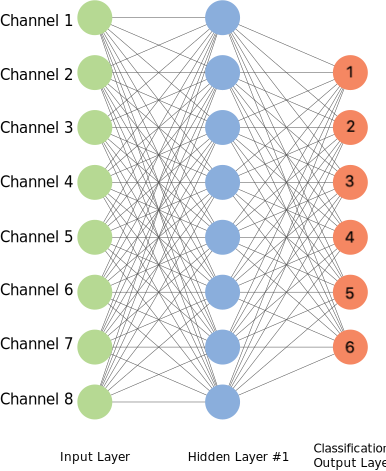
\includegraphics[width=.9\linewidth]{Graphics/1-layer-NN}
  \caption{Schematic of input hidden and classification layers of ANN with all 8 channels as input}
  \label{fig:1Layer}
\end{subfigure}%
\begin{subfigure}{.6\textwidth}
  \centering
  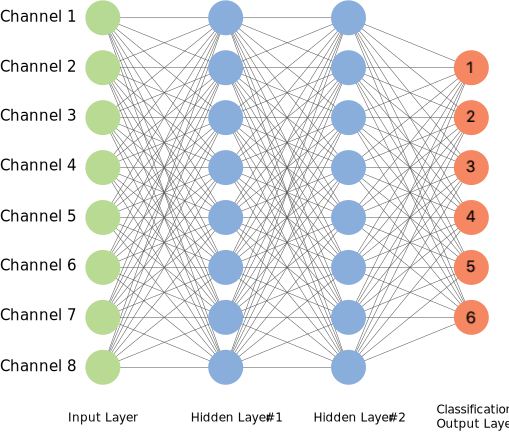
\includegraphics[width=.9\linewidth]{Graphics/2-layer-NN}
  \caption{Schematic of input hidden and classification layers of ANN with 4 principle components as input}
  \label{fig:2Layer}
\end{subfigure}
\caption{Neuronal Net structures}
\label{gig:Model}
\end{figure}

To create the computation graphs for the ANN we used the R implementation of Keras which relies on Google's TensorFlow engine for backpropogation. This allows us to add, edit, and remove layers from our models as needed during the development process. The flexibility of this modular design means we are able to prototype new models quickly.

\begin{com}
To assess the performance of each ANN, we used an $80/20$ split our data to generate a gesture-specific training and a testing sets. These were done automatically in the Keras package via random sampling. We then assessed the classifcation accuracy of each ANN using a categorical cross entropy metric which measures the \textit{Kullback-Leibler} (KL) divergence between the true distribution of the response variable and the distribution of the predictions.
\end{com}

\section{Results}

\subsection{Principal Component Analysis}

Using the spectral decomposition we found that only $4$ of the $8$ principal components in our dataset contributed meaningfully to variance in our response. From figure $3$, we can see that these $4$ components account for approximately $80$\% of the variability we are seeking to model.


\begin{figure}[H]
  \centering
  \caption{PCA Screeplot and cumulutive variance plot}
  \includegraphics[width=0.9\textwidth]%
    {Graphics/PCA_Plots/PCA_screeplot-150dpi}% picture filename
    \label{fig:PCA}
\end{figure}


By reducing the number of inputs from $8$ smoothed signals to only $4$ principle components, we were able to reduce overfitting in our model prior to ultizing any dropout layers. This reduction in overfitting decreased prediction accuracy in the validation data set only slightly see the \textit{ANN Performance Comparison} section.


\subsection{ANN Performance Comparison}


\begin{center}
-- Predictive Accuracy Using $8$ Smoothed Channels --\\

-- Predictive Accuracy Using $4$ Principle Components --
\end{center}



\newpage





\section*{References}


\bibliographystyle{apacite}
\bibliography{References}



\end{document}
